
\documentclass{beamer}
\usepackage{pgfpages}
\usepackage[T2A]{fontenc}
\usepackage[cp1251]{inputenc}
\usepackage[english]{babel}
\usepackage{study}
\usepackage{hyperref}

\title[Introduction]{ \large{\textsf{Software Engineering}}\\[10mm]%
  Introduction}
\author{Sasha Shapoval}
\institute[UoL]{University of Lodz}
\date{February 27, 2024}
\mode<presentation>
{
  \usetheme{Madrid}
  \setbeamercovered{transparent}
  \usefonttheme[stillsansseriflarge]{serif}
}

\usecolortheme[named=brown]{structure}


\begin{document}

\begin{frame}
  \maketitle
\end{frame}

\begin{frame}{Grading}
The grades of the course consist of the grades for the intermediate elements of control and the final exam. The weights are $0.6$ and $0.4$ respectively. Note that the marks for the group project are individual. The project topic and the contribution of each team member are agreed at the beginning. The formula is
\[
  Grade =
  \verbcode{round}(0.4 \times \mathrm{\mathrm{\text{``}Exam\text{''}}} +
    0.15 \times \mathrm{T}
    +
    0.1 \times \mathrm{P1}
    +
    0.15 \times \mathrm{P2}
    +
    0.20 \times \mathrm{P3}
  )
\]
where $T$ and $P$ stands for the test and presentations respectively.
Rounding is to available grades: $2$, $3$, $3.5$, $4$, $4.5$, $5$.
\end{frame}

\begin{frame}{Dates of the elements of control}
  \begin{itemize}
    \item
      Test: 11.03--15.03 (according to the group schedule)
    \item
      Presentation 1: 08.04--12.04
    \item
      Presentation 2: 05.05--09.05
    \item
      Presentation 3: 26.05--30.05
    \item
      Exam: 09.06--13.06
  \end{itemize}
  \begin{block}{Office Hours}
    \begin{itemize}
      \item
	Wednesday, 16:15--17:45
      \item
	Office hours are for questions; NO elements of control are passed during office hours
    \end{itemize}
  \end{block}
\end{frame}

\begin{frame}{Elements of control: Test}
  \begin{itemize}
    \item
      Four tasks (university computers; internet off)
    \item
      Basic elements of algorithms: operations with integers, lists, loops
    \item
      Basic drawing with \texttt{turtle}.
  \end{itemize}
\end{frame}

\begin{frame}{Elements of control: Presentation 1}
  \begin{itemize}
    \item
      Introductory presentation of the project with grading for
    \item
      Understanding of basic models of software engineering and team building by using your team and the project as examples (in particular you have to specify who does what)
    \item
      ``Selling`` the brief of your project (imitate that you offer a project for investors)
    \item
      Explanation of basic ideas, main challenges, and \textbf{links} between the different project parts (performed by different team members). In particular, you present the skeleton of your code (single slide)
    \item
      Ability to meet the time constrain of $12$ minutes for the presentation
  \end{itemize}
\end{frame}

\begin{frame}{Elements of control: Presentation 2}
  \begin{itemize}
    \item
      Presentation introducing a workable code with grading for
    \item
      Code itself (main challenge and the way to overcome)
    \item
      Explanation of the links between your part of the code and the other parts
    \item
      Ability to meet the time constrain of $12$ minutes for the presentation
    \item
      Note: the speaker who cannot answer questions about the meaning of the lines of their code gets mark $0$ for this presentation
  \end{itemize}
\end{frame}

\begin{frame}{Elements of control: Presentation 3}
  \begin{itemize}
    \item
      Final presentation with grading for
    \item
      Explanation of the context (the aim of the project, known approach to the problem, system requirements)
    \item
      Workability of the project
    \item
      Ability to meet the time constrain of $12$ minutes for the presentation
  \end{itemize}
\end{frame}

\begin{frame}{Possible Project Components: $3$ are mandatory}
\begin{enumerate}
  \item
    simple drawing (\texttt{turtle}, \texttt{tkinter})
  \item
    parsing of web-pages (\texttt{BeautifulSoup})
  \item
    processing of numerical data that includes the computation of relevant statistics (\texttt{pandas}, \texttt{numpy}, \texttt{scikit-learn}
  \item
    more advanced previous item that includes the verification of a statistical hypothesis
  \item
    visualization of numerical data (\texttt{matplotlib}, \texttt{seaborn}, \texttt{plotly}
  \item
    backend with a (telegram) bot (\texttt{pytelegrambotapi})
  \item
    testing (\texttt{unittest} + test as you go)
\end{enumerate}
\end{frame}

\begin{frame}{Recommended projects}
  \begin{itemize}
    \item
      Educational games (labyrinths, race to $100$, Hanoi tower), where computation part is shared with you, and other things like leader board, audio and visual effect, and the backend can be added
    \item
      Parsing of the sites with numerical data followed by the data processing to graphical representation of the output and the control of requests through a messenger (you will have the codes that parse a site with the Covid data manipulating the extracted numbers, processing of the Bitcoin data, and drawing the graphs)
    \item
      Prediction of time series, where the input is given as a file (you may use the interpolation / extrapolation techniques and examples of visualization discussed in the class); backend with a messenger can complement the project
    \item
      Other projects that meet the requirements and agreed with the lecturer
  \end{itemize}
\end{frame}

\begin{frame}{General notes on projects}
  \begin{itemize}
    \item
      I grade for the projects that show your knowledge of the course. All codes used in the course are shared with you
    \item
      You can get at least $4.5$ out of $5$ for a simple workable project based on the codes that I share with you
    \item
      You may decide to \emph{improve} a basic project adding the elements not studied within our course
    \item
      These additional elements are not graded without the demonstration of knowledge related to the course
  \end{itemize}
\end{frame}

\begin{frame}{Elements of control: Exam}
  \begin{itemize}
    \item
      $5$ tasks, $1$ question about theory of software engineering, $4$ questions that require to write a code to answer
    \item
      Lab computers, Internet off, materials can be saved to the laboratory computer in advance
    \item
      No new questions
  \end{itemize}
\end{frame}

\begin{frame}{Students' Comments (2023)}
  \begin{itemize}
    \item
      Professor has inbuilt scanner detecting only those student who does not know anything about the project
    \item
      Should behave equally with every student:
      \emph{I spent too much time for bad projects making everybody clear that the work has not been performed properly; will change}
    \item
      Some actual coding would be nice
    \item
      exam + huge team project is too much
      \emph{Please note, I do not require huge project; I am asking for a workable (mock) project}
  \end{itemize}
\end{frame}

\begin{frame}{Python}
  \begin{itemize}
    \item 
      For most platforms, you can download the required installation files from
      \url{https://www.python.org/downloads/} and install them using the appropriate platform-specific method
    \item
      You can use cloud resource Colab, which is an online Jupyter Notebook environment from Google: \url{https://colab.research.google.com/}.
      It is strongly recommended because the resource simplifies the presentation of your projects in the class
    \item
      Jupyter Notebook for your personal computer is recommended within Anaconda (\url{https://anaconda.org/})
  \end{itemize}
\end{frame}

\begin{frame}{Course Parts}
  \begin{itemize}
    \item 
      Management: team building, the efficiency of the projects
    \item
      Software: (presumably efficient) coding
    \item
      Algorithms
    \item
      Elementary mathematics (mostly, probability and statistics) only to use library functions
  \end{itemize}
\end{frame}

\begin{frame}{Course materials}
  \begin{itemize}
    \item
      Roger S. Pressman
      Software engineering: a practitioner�s approach
    \item
      Lecture notes
    \item
      Allen B. Downey, Think Stats Probability and Statistics for Programmers
      \url{https://greenteapress.com/thinkstats/}\\
      codes: \url{https://greenteapress.com/thinkstats/thinkstats.code.zip}\\
      data: \url{https://greenteapress.com/thinkstats/nsfg.html}
    \item
      Jake VanderPlas, Python data science handbook,\\
      github with everything: \url{https://github.com/jakevdp/PythonDataScienceHandbook}\\
      handbook only: \url{https://jakevdp.github.io/PythonDataScienceHandbook/}
  \end{itemize}
\end{frame}

\begin{frame}{Introducing myself}
  \begin{itemize}
    \item
      \href{https://sashashapoval.github.io/}{{\color{blue}Professor Sasha (Alexander) Shapoval}}
    \item 
      Researcher with background in mathematics and computer science
    \item
      Fields of interests: complex systems, data analysis, prediction of extremes, mathematical economics
    \item
      Papers in international refereed journals including
      \emph{Scientific Reports},
      \emph{Physica D},
      \emph{Astrophysical Journal}
      \emph{Communications in Nonlinear Science and Numerical Simulation},
      \emph{Journal of Mathematical Economics}
    \item
      Research grants
    \item
      Cooperation with industry as an expert in projects
  \end{itemize}
\end{frame}

\begin{frame}[<+->]{Value one's time}
  \begin{itemize}
    \item
      Send emails, do not chat
    \item
      Structure your presentation to make it useful for listeners
    \item
      Unfortunately, presenters care about listeners rarely. The schedule is organized in advance
    \item
      I will set the order of presentations following my list. If you want another order, cooperate
    \item
      Use messengers to cooperate, e.~g., telegram
    \item
      In exceptional cases, online cooperation with me is possible
  \end{itemize}
\end{frame}

\begin{frame}[<+->]{Why do we study this course}
  \begin{itemize}
    \item
      This is the (part of the) profession
    \item
      Open linkedin and look for data analyst, software developes, quantitative analysis and you see our topics as the requirements
  \end{itemize}
\end{frame}

\begin{frame}[<+->]{Following the book focused on management}
  \textit{Roger S. Pressman},
  Software engineering: a practitioner�s approach
\end{frame}

\begin{frame}[<+->]{Summary / Topics / Questions}
  \begin{itemize}
    \item
      What is my name?
    \item
      What is the title of the course
    \item
      How are the final grades calculated? What are the elements of control?
    \item
      What are the dates of the presentations, test, and exam?
    \item
      What are the requirements to the project?
    \item
      What is the attitude to cheating?
  \end{itemize}
\end{frame}

\begin{frame}[<+->]{Software engineering is}
  \begin{block}{Fritz Bauer (1969)}
    the establishment and use of sound engineering principles in
    order to obtain economically sounding software that is reliable and works efficiently on real machines
  \end{block}
  \begin{block}{}
    \begin{itemize}
      \item 
	The application of a systematic, disciplined, quantifiable approach to the development, operation, and maintenance of software; that is, the application of engineering to software
      \item
	The study of approaches as in the previous item
    \end{itemize}
  \end{block}
\end{frame}

\begin{frame}{}
  \visible<+->{\begin{block}{Components of Software Engineering}
    \hbox to \hsize{\hfil
      
\includegraphics[width = 0.8\textwidth]{scheme.jpg}
    \hfil}
  \end{block}}
  \visible<+->{\begin{block}{Components of Software Engineering}
      \begin{itemize}
	\item 
	  What are these components in the creation of USOS-system of the University of Lodz
	\item
	  of Visual Studio Code?
	\item
	  in the definition of a class in \texttt{C++}?
      \end{itemize}
  \end{block}}
\end{frame}

\begin{frame}[<+->]{Parts of Software Engineering}
  \begin{itemize}
    \item 
      definition phase: what must be done
    \item
      development phase: how it can be done
    \item
      support phase: correction of errors
  \end{itemize}
\end{frame}

\begin{frame}{Definition phase}
  \begin{itemize}
    \item 
      During definition, the software engineer attempts to identify what information is to be processed, what function and performance are desired, what system behavior can be expected, what interfaces are to be established, what design constraints exist, and what validation criteria are required to define a successful system.
    \item
      The key requirements of the system and the software are identified. Although the methods applied during the definition phase will vary depending on the software engineering paradigm (or combination of paradigms) that is applied, three major tasks will occur in some form: system or information engineering, software project planning, and requirements analysis.
  \end{itemize}
\end{frame}

\begin{frame}{Developmet phase}
  \visible<+->{\begin{block}{}during development a software
engineer attempts to define how data are to be structured, how function is to be implemented within a software architecture, how procedural details are to be implemented, how interfaces are to be characterized, how the design will be translated into a programming language (or nonprocedural language), and how testing will be performed. The methods applied during the development phase will vary, but three specific technical tasks should always occur: software design, code generation, and software testing.
  \end{block}}
  \visible<+->{\begin{block}{}%
    Can you describe different stages at the marshmallow challenge?\\
    Can you associate testing with any stage of the marshmallow challenge?
  \end{block}}
\end{frame}

\begin{frame}{The support phase}
  \visible<+->{\begin{block}{}focuses on change associated with error correction, adaptations required as the software's environment evolves, and changes due to enhancements brought about by changing customer requirements. The support phase reapplies the steps of the definition and development phases but does so in the context of existing software\end{block}}

  \visible<+->{\begin{block}{}%
    you bought a computer with Windows and got the support that would last forever; for how long will this forever last?
  \end{block}}

  \visible<+->{\begin{block}{}%
    What do you expect from the developers of Windows?\\
    To what extent your expectations are met?
  \end{block}}
\end{frame}

\begin{frame}{Classic lifecyle or waterfall model}
  \visible<+->{\begin{block}{Scheme}
    \hbox to \hsize{\hfil
      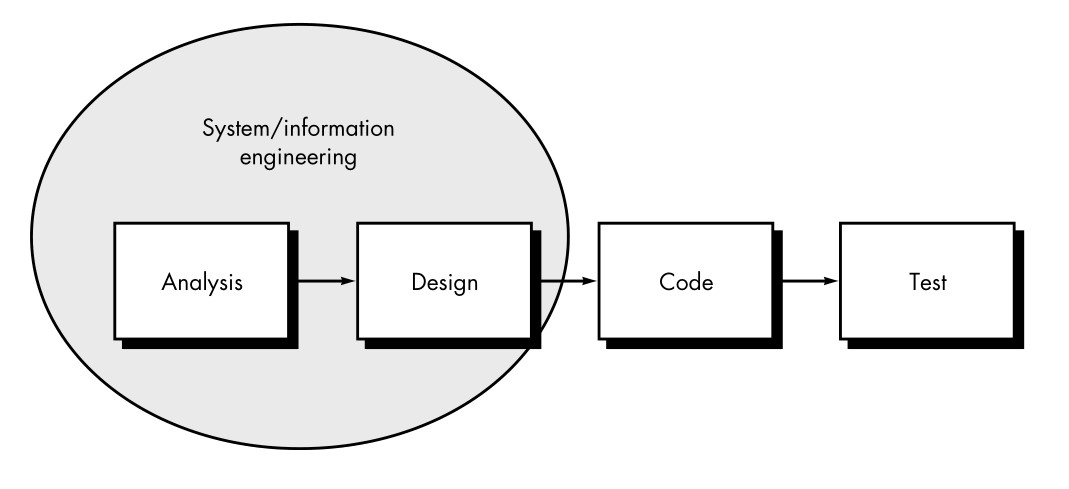
\includegraphics[width = 0.8\textwidth]{waterfall.jpg}
    \hfil}
  \end{block}}
  \visible<+->{\begin{block}{}
      \visible<.->{Is this scheme applicable to Windows?}\\
      \visible<+->{Rather not as the processes go in parallel and are repeated many times}\\
      \visible<.->{Is this scheme applicable to simple drawing project?}\\
      \visible<.->{Rather, yes because of its simplicity}
  \end{block}}
\end{frame}

\begin{frame}{Software requirements analysis}
  The requirements gathering process is intensified and focused specifically on software. To understand the nature of the program(s) to be built, the software engineer must understand the information domain for the software, as well as required function, behavior, performance, and interface. Requirements for both the system and the software are documented and reviewed with the customer.
\end{frame}

\begin{frame}{Design}
  Software design is actually a multi-step process that focuses on four distinct attributes of a program: data structure, software architecture, interface representations, and procedural (algorithmic) detail. The design process translates requirements into a representation of the software that can be assessed for quality before coding begins. Like requirements, the design is documented and becomes part of the software configuration
\end{frame}

\begin{frame}{Code generation}
  The design must be translated into a machine-readable form. The code generation step performs this task. If design is performed in a detailed manner, code generation can be accomplished mechanistically.
\end{frame}

\begin{frame}{Testing}
  Once code has been generated, program testing begins. The testing process focuses on the logical internals of the software, ensuring that all statements have been tested, and on the functional externals; that is, conducting tests to uncover errors and ensure that defined input will produce actual results that agree with required results.
\end{frame}

\begin{frame}{Support}
  Software will undoubtedly undergo change after it is delivered to the customer (a possible exception is embedded software). Change will occur because
\begin{itemize}
  \item 
    errors have been encountered,
  \item
    the software must be adapted to accommodate changes in its external environment (e.g., a change required because of a new operating system or peripheral device)
  \item
    the customer requires functional or performance enhancements
\end{itemize}
   Software support/maintenance reapplies each of the preceding phases to an existing program rather than a new one.
\end{frame}

\begin{frame}{Prototyping model: Scheme}
  \begin{block}{}
    \hbox to \hsize{\hfil
      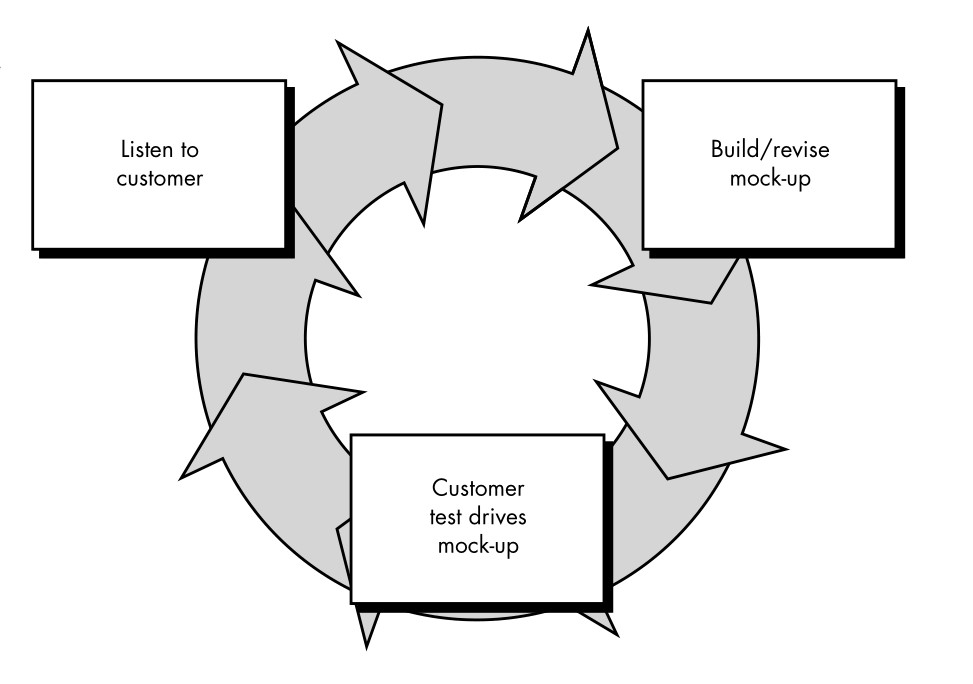
\includegraphics[width = 0.5\textwidth]{prototype.jpg}
    \hfil}
  \end{block}
  \visible<+->{\begin{block}{}
      \visible<.->{Is this scheme applicable to windows?}\\
      \visible<+->{Probably, yes, but to what extent the developers follow the customers}\\
      \visible<+->{Is this scheme applicable to such open source projects as C or Python language themselves and their environments?}\\
      \visible<+->{Likely, yes, but who receives profits from the project and how?}
  \end{block}}
\end{frame}

\begin{frame}{Prototyping model}
  \begin{itemize}
    \item requirements gathering: obtained from customers
    \item
      Then the prototype is evaluated by the customer/user and used to refine requirements for the software to be developed.
  \end{itemize}
\end{frame}

\begin{frame}{Other models}
  \begin{itemize}
    \item 
      Rapid application development
    \item
      Evolutionary software process models
      \begin{itemize}
	\item
	  spiral model
	\item
	  Concurrent Development Model
      \end{itemize}
    \item
      Formal methods model
    \item
      Fourth generation techniques
  \end{itemize}
\end{frame}

\begin{frame}{Fourth generation techniques}
  The term fourth generation techniques (4GT) encompasses a broad array of software tools that have one thing in common: each enables the software engineer to specify some characteristic of software at a high level. The tool then automatically generates source code based on the developer's specification. There is little debate that the higher the level at which software can be specified to a machine, the faster a program can be built. The 4GT paradigm for software engineering focuses on the ability to specify software using specialized language forms or a graphic notation that describes the problem to be solved in terms that the customer can understand.
\end{frame}

\begin{frame}{Fourth generation techniques}
  Currently, a software development environment that supports the 4GT paradigm includes some or all of the following tools:
  \begin{itemize}
    \item
      nonprocedural languages for database query
    \item
      report generation, data manipulation, screen interaction and definition, code generation
    \item
      high-level graphics capability;
    \item
      spreadsheet capability, and automated generation of HTML and similar languages used for Web-site creation using advanced software tools.
  \end{itemize}
  Initially, many of the tools noted previously were available only for very specific application domains, but today 4GT environments have been extended to address most software application categories.
\end{frame}

\end{document}

